\documentclass[11pt]{article}

% Invoke with
% pdflatex -jobname final-solutions "\def\showkey{}\documentclass[11pt]{article}

% Invoke with
% pdflatex -jobname final-solutions "\def\showkey{}\documentclass[11pt]{article}

% Invoke with
% pdflatex -jobname final-solutions "\def\showkey{}\documentclass[11pt]{article}

% Invoke with
% pdflatex -jobname final-solutions "\def\showkey{}\input{final.tex }"
% for solutions


% Compiler structure
% Scanning: RE, DFA, NFA, Subset construction
% Parsing: SLR table, shift/reduce parsing, First and Follow
% Types: arrays, structs and unions, static typing, polymorphism
% Runtime: activation records, recursion, variable-sized arrays, access links
%   Layout of structs, unions, arrays, malloc, reference counting, mark/sweep
%   Objects, inheritance, virtual functions
%   setjmp/longjmp, exceptions
% Code Generation: stack vs. register-based IRs, CFGs, optimization, linking
% Lambda Calculus: beta reduction, alpha conversion, normal form, Church-Rosser
%   Booleans, Church Numerals, Recursion and the Y combinator
% Prolog: Horn clauses, structures and functors, unification,
%   recursive searching, cuts

% ``Dismantle the following program into gotos, etc.''
% What does this Prolog program do?
% Strict functions and applicative order evaluation: what does this do?
% Unfamiliar language: scoping rules, applicative or normal order,

% Simple RE:
%
%  Draw NFA
%  Show parse of a string
%  Convert to DFA subset construction
%  Show parse of 
% 

% http://jsmachines.sourceforge.net/machines/slr.html
% Very simple grammar:
%
% E' -> E
% E -> ( E )
% E -> id
%
% six states
%
% Parse ( ( id ) )
%   steps: s2 s2 s3 r2 s5 r1 s5 r1
% 
%  Draw LR(0) automaton
%  First and follow sets
%  Fill in parse table
%  Parse simple input

% Draw parse trees for each way this expression could be parsed
%   Lambda calculus example

% Ocaml:
%   Is it applicative or normal?
%   Give a program, say it does this or that, and ask whether it's applicative
%   or normal
%
%   Can it use a stack for its activation records?
%    Simple example (yes)
%    Example that returns a lambda (no)


% Disambiguate a grammar by restructuring it
%
% E -> E + E | E ^ E | ( E ) | num
%
% make + left associative, ^ right associative, and + at a lower precedence
%
% E -> E + T | T
% T -> F ^ T | F
% F -> ( E ) | num

% Evaluate this lambda term using normal-order evaluation
%   " using applicative order evaluation

\usepackage[T1]{fontenc}
\usepackage{fourier}
\usepackage[scaled=0.88]{luximono}
\usepackage{booktabs}
\usepackage{array}
\usepackage{tikz}
\usetikzlibrary{positioning,calc,automata}
\usepackage{listings}
\lstset{basicstyle=\ttfamily}

{\obeyspaces\global\let =\ }
\newenvironment{lcalc}{\begingroup$\obeyspaces\begin{array}{r@{\;}c@{\;}l}}{\end{array}$\endgroup}

\newif\ifkey

%\def\showkey{}

\ifdefined\showkey
  \keytrue
\else
  \keyfalse
\fi

\newcommand{\key}[1]{\ifkey\rlap{\quad\textcolor{red}{#1}}\fi}

\newcommand{\fillinbox}[1][X]{%
  \framebox[3pc]{\rule[-1.2pc]{0pt}{3pc}\ifkey \textcolor{red}{\Large #1} \fi}\hspace{5pt}}

\makeatletter
\newcommand\listofproblems{
  \problemline{\textbf{Problem}}{\textbf{Value}}{\textbf{Score}}{\textbf{Description}}
  \@starttoc{lop}
  \problemline{Total}{\arabic{total}}{}{}
}
\makeatother

\def\labelenumi{\alph{enumi})}

\def\problemline#1#2#3#4{\noindent\par\hspace{10pc}\hbox{\hbox to 3.5pc{\hfil#1\hfil}\hbox to 3pc{\hfil#2\hfil}\hbox to 6pc{\hfil#3\hfil}\hbox{#4}}\par\noindent\hspace{10pc}\rule{23pc}{0.5pt}}

\def\problemspec#1#2#3#4{\problemline{#1}{#2}{#3}{#4}
\addtocounter{total}{#2}}

\newcounter{problem}
\newenvironment{problem}[2]{
  \refstepcounter{problem}
  \par\noindent
  \arabic{problem}. (#1 pts.)
  \addtocontents{lop}{\protect\problemspec{\theproblem}{#1}{}{#2}}
}

\newcounter{total}

% Make ``.'' a mathrel symbol: improves spacing in lambda expressions
\mathcode`\.="313A
% Make | a mathrel symbol
\mathcode`\|="326A

\tikzset{>=latex} % Nicer looking arrows

\usepackage[top=0.5in,bottom=1in,left=0.5in,right=0.5in]{geometry}

\def\kleene#1#2#3#4{
  \path [->] (#1) edge node [above] {$\epsilon$} (#2)
             (#3) edge node [above] {$\epsilon$} (#4)
             (#3) edge [bend right=60] node [above] {$\epsilon$} (#2)
             (#1) edge [bend right] node [below] {$\epsilon$} (#4)
  ;
}
\def\choice#1#2#3#4#5#6{
  \path [->] (#1) edge node [above] {$\epsilon$} (#2)
             (#1) edge node [below] {$\epsilon$} (#3)
             (#4) edge node [above] {$\epsilon$} (#6)
             (#5) edge node [below] {$\epsilon$} (#6)
  ;
}
\def\single#1#2#3{
  \path [->] (#1) edge node [above] {#3} (#2);
}

\newcommand{\myfbox}[3]{
  \fbox{\begin{minipage}[t][#2]{#1}\mbox{}#3\end{minipage}}
}

\newcommand{\field}[3]{
  \myfbox{#1}{#2}{\ifkey{\color{red}#3}\fi}
}

\def\fullfield{\field{\textwidth}}

\title{COMS W4115 Programming Languages and Translators Final}
\author{ Prof. Stephen A. Edwards \quad\quad December 10, 2018}
\date{}

\begin{document}
\maketitle

Name: \begin{tabular}{@{}c@{}}\field{30pc}{1.5pc}{Key}\end{tabular}
Uni: \begin{tabular}{@{}c@{}}\field{5pc}{1.5pc}{}\end{tabular}


{\parskip=0.5\baselineskip

  75 minutes
  
You may consult your own 8.5$''$ $\times$ 11$''$ double-sided sheet of
notes, but nothing else (e.g., no text, no other notes).

You may use a four-function calculator, but probably don't need one.

Put your answers in the boxes provided; writing outside the
boxes will not be graded.  Use scratch paper if necessary.

Explain your answers.

Check this box if you are \textbf{not enrolled} in the class (i.e.,
taking the comp exam)
\hspace{1pc}
\begin{tabular}{@{}c@{}}\field{0.7pc}{0.7pc}{}
\end{tabular}
}

\vspace{3pc}

%\listofproblems

% http://hackingoff.com/compilers/regular-expression-to-nfa-dfa

\begin{problem}{12}{Grammar Disambiguation}
Write an \textbf{unambiguous grammar} for the language defined by the
following ambiguous grammar by making the $+$ operator
\textbf{left-associative} and the $\wedge$ operator
\textbf{right-associative} at a \textbf{higher level of precedence}
than $+$. The terminals are $+$, $\wedge$, $($, $)$, and $n$.  $|$
indicates choice.

\[
E \rightarrow E + E | E \wedge E | (\ E\ ) | n
\]

\noindent\fullfield{2.5in}{
\[
\begin{array}{l}
E \rightarrow E + T \\
E \rightarrow T \\
T \rightarrow F \wedge T \\
T \rightarrow F \\
F \rightarrow ( E ) \\
F \rightarrow n
\end{array}
\]
}

\end{problem}

\newpage

\begin{problem}{20}{Regular Expressions}
\begin{enumerate}
\item (5 pts.) Using Thompson's construction (from class),
  \textbf{draw the NFA} for the regular expression $a^*|(b^*|c^*)$

\hspace{-2.5pc}\fullfield{2.75in}{
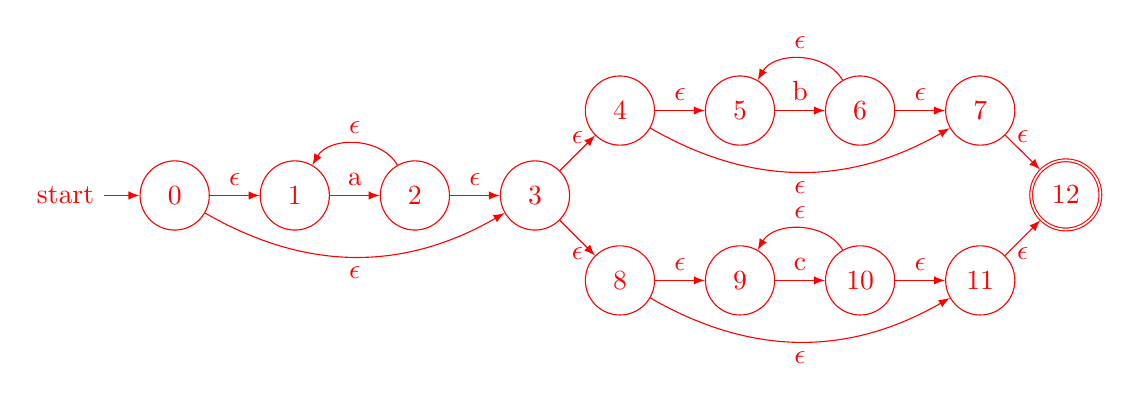
\begin{tikzpicture}[node distance=1.5pc,color=red]
\node[state,initial] (0) {0};
\node[state,right=of 0] (1) {1};
\node[state,right=of 1] (2) {2};
\node[state,right=of 2] (3) {3};
\node[state,above right=of 3] (4) {4};
\node[state,right=of 4] (5) {5};
\node[state,right=of 5] (6) {6};
\node[state,right=of 6] (7) {7};
\node[state,below right=of 3] (8) {8};
\node[state,right=of 8] (9) {9};
\node[state,right=of 9] (10) {10};
\node[state,right=of 10] (11) {11};
\node[state,accepting,above right=of 11] (12) {12};
\kleene 0 1 2 3
\single 1 2 a
\choice 3 4 8 7 {11} {12}
\kleene 4 5 6 7
\single 5 6 b
\kleene 8 9 {10} {11}
\single 9 {10} c
\end{tikzpicture}
}

\item (5 pts.) Convert the NFA you wrote in part (a) to a \textbf{DFA} using
  the \textbf{subset construction algorithm.}  \textbf{Fill in the table} below
  to show how you arrived at your DFA and \textbf{draw the DFA}.

  \hspace{-2.5pc}\myfbox{\textwidth}{2.75in}{
\renewcommand{\arraystretch}{1.5}\large
\ifkey\color{red}\fi
\begin{tabular}[b]{cp{14pc}ccc}
\toprule
\multicolumn{2}{@{}c@{}}{\textbf{Current State}} &
\multicolumn{3}{@{}c@{}}{\textbf{Next State}} \\
\cmidrule(r){1-2}
\cmidrule(l){3-5}
\textbf{DFA} &
\multicolumn{1}{@{\hspace{8pc}}c@{\hspace{8pc}}}{\textbf{NFA States}} &
\textbf{a} &
\textbf{b} &
\textbf{c} \\
\midrule
\ifkey
A & \{ 0, 1, 3, 4, 5, 7, 8, 9, 11, 12 \} & B & C & D \\
B & \{ 1, 2, 3, 4, 5, 7, 8, 9, 11, 12 \} & B & C & D  \\
C & \{ 5, 6, 7, 12 \} & & C & \\
D & \{ 9, 10, 11, 12 \} & & & D \\
\else
\\
\fi
\end{tabular}
\ifkey
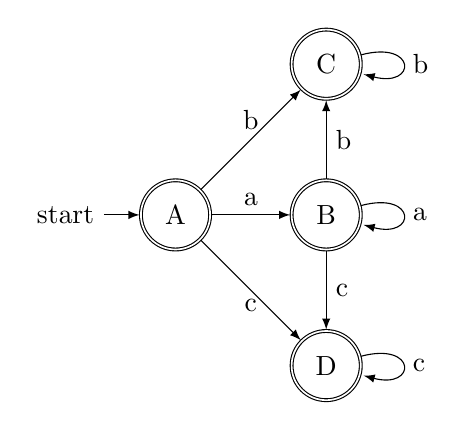
\begin{tikzpicture}
\node [state,initial,accepting] (A) {A};
\node [state,right=of A,accepting] (B) {B};
\node [state,above=of B,accepting] (C) {C};
\node [state,below=of B,accepting] (D) {D};
\path [->] (A) edge node [above] {a} (B)
           (A) edge node [above] {b} (C)
           (A) edge node [below] {c} (D)
           (B) edge node [right] {b} (C)
           (B) edge node [right] {c} (D)
           (B) edge [loop right] node [right] {a} ()
           (C) edge [loop right] node [right] {b} ()
           (D) edge [loop right] node [right] {c} ()
;
\end{tikzpicture}
\fi
}


\item (5 pts.) Show how your NFA from part (a) \textbf{accepts the
  string} $bb$ by indicating the \textbf{sequence of states} it goes
  through.

\def\trans#1{\buildrel{#1}\over\rightarrow}
\def\ep{\rightarrow}

\hspace{-2.5pc}\fullfield{0.5in}{
$0 \ep 3 \ep 4 \ep 5 \trans b 6 \ep 5 \trans b 6 \ep 7 \ep 12$
}

\item (5 pts.) Show how your DFA from part (b) \textbf{accepts the
  string} $bb$ by indicating the \textbf{sequence of states} it goes
  through.

\hspace{-2.5pc}\fullfield{0.5in}{
$A \trans b C \trans b C$
}

\end{enumerate}
\end{problem}

\newpage

\begin{problem}{8}{Normal vs. Applicative}

For the lambda term $(\lambda x . \lambda y . +\ y\ y)\ \big((\lambda z . z\ z)\ (\lambda w . w\ w)\big)$

\begin{enumerate}
\item (4 pts.) \textbf{Show the steps} in reducing this term to normal form, if
  possible, using \textbf{normal-order evaluation}. \\
  \textbf{Underline} the complete subexpression being $\beta$-reduced.

\hspace{-2.5pc}\fullfield{1.75in}{
$\underline{(\lambda x . \lambda y . +\ y\ y)\ \big((\lambda z . z\ z)\ (\lambda w . w\ w)\big)}$ 

$(\lambda y . +\ y\ y)$
}

\item (4 pts.) \textbf{Show the steps} in reducing this term to normal form, if
  possible, using \textbf{applicative order evaluation}.
  \textbf{Underline} each subexpression being $\beta$-reduced.

  \hspace{-2.5pc}\fullfield{1.75in}{
    $(\lambda x . \lambda y . +\ y\ y)\ \big(\underline{(\lambda z . z\ z)\ (\lambda w . w\ w)}\big)$


$(\lambda x . \lambda y . +\ y\ y)\ \big(\underline{(\lambda w . w\ w)\ (\lambda w . w\ w)}\big)$ 

Etc. Does not ever normalize.
}

\end{enumerate}

\end{problem}

\begin{problem}{15}{Church Numerals}
Recall the Church Numerals and the ``plus'' function, which adds \emph{m} to \emph{n}:

\medskip

\begin{lcalc}
0 & = & \lambda{f} . \lambda{x} . x \\
1 & = & \lambda{f} . \lambda{x} . f x \\
\end{lcalc}
\hfil
\begin{lcalc}
2 & = & \lambda{f} . \lambda{x} . f (f x) \\
3 & = & \lambda{f} . \lambda{x} . f \big(f (f x)\big) \\
\end{lcalc}
\hfil
\begin{lcalc}
\textrm{plus} & = & \lambda{m}.\lambda{n}.\lambda{f}.\lambda{x}. m f ( n f x)
\end{lcalc}

\medskip

\textbf{Prove} that in the Lambda Calculus, $\textrm{plus}\ 1\ 1 =
2$. \textbf{Justify} each step of your proof.

\noindent\fullfield{3in}{
\begin{lcalc}
\textrm{plus} 1 1 & = & (\lambda{m}.\lambda{n}.\lambda{f}.\lambda{x}. m f ( n f x)) 1 1 \\
& =_{\beta} & \lambda{f}.\lambda{x}. 1 f ( 1 f x )  \\
& = & \lambda{f}.\lambda{x}. 1 f ( (\lambda{f}. \lambda{x}. f x) f x ) \\
& =_{\beta} & \lambda{f}.\lambda{x}. 1 f ( f x ) \\
& = & \lambda{f}.\lambda{x}. (\lambda{f}. \lambda{x}. f x) f ( f x ) \\
& =_{\beta} & \lambda{f}.\lambda{x}. f ( f x ) \\
& = & 2 \\
\end{lcalc}
}


\end{problem}

\begin{problem}{25}{Parsers}
For the grammar \quad $\begin{array}{l}
E' \rightarrow E \\
E \rightarrow (\ E\ ) \\
E \rightarrow a
\end{array}$ \quad whose three terminals are (, ), and a.

\begin{enumerate}

\item (10 pts.) Complete its LR(0) automaton. Fill in the \textbf{items},
  indicate the \textbf{accepting states}, and label the
  \textbf{transitions}.  No additional transitions are necessary.

\newcommand{\itemtab}[1]{
  \ifkey{\color{red}
  \begin{tabular}{>{$}l<{$}@{\ $\rightarrow$\ }>{$}l<{$}} #1 
  \end{tabular}
}\fi}

\newcommand{\lab}[1]{\ifkey\textcolor{red}{#1}\fi}

\begin{tikzpicture}
\node [draw,minimum height=6pc,text width=10pc] (S0) {\itemtab{
E' & \cdot E \\
E & \cdot (\ E\ ) \\
E & \cdot a \\
}};

\node [draw,minimum height=6pc,text width=10pc,right=of S0] (S1) {\itemtab{
E' & E \cdot \\
}};

\node [draw,minimum height=6pc,text width=10pc,below right=of S0] (S2) {\itemtab{
E & ( \cdot E \ ) \\
E & \cdot (\ E\ ) \\
E & \cdot a \\
}};

\node [draw,minimum height=6pc,text width=10pc,left=of S2] (S3) {\itemtab{
E & a \cdot \\
}};

\node [draw,minimum height=6pc,text width=10pc,right=of S2,xshift=2pc] (S4) {\itemtab{
E & (\ E \cdot ) \\
}};

\node [draw,minimum height=6pc,text width=10pc,above=of S4] (S5) {\itemtab{
E & (\ E \ ) \cdot \\
}};

\node [below left] at (S0.north west) {S1};
\node [below left] at (S1.north west) {S6};
\node [below left] at (S2.north west) {S2};
\node [below left] at (S3.north west) {S3};
\node [below left] at (S4.north west) {S4};
\node [below left] at (S5.north west) {S5};

\path [<-] (S0.west) edge ++(left:0.5);

\path [->] (S0) edge node [above] {\lab E} (S1);
\path [->] (S0) edge node [above] {\lab (} (S2);
\path [->] (S0) edge node [right] {\lab{a}} (S3);
\path [->] (S2) edge [in=25,out=35,loop] node [right] {\lab (} ();
\path [->] (S2) edge node [above] {\lab{a}} (S3);
\path [->] (S2) edge node [above] {\lab{E}} (S4);
\path [->] (S4) edge node [right] {\lab )} (S5);

\end{tikzpicture}


\item (5 pts.) \textbf{Compute} the \textsc{first} and \textsc{follow} sets.  \textbf{Explain} your reasoning.

  \hspace{-2.5pc}\myfbox{\textwidth}{1.5in}{
\parskip=6pt

$\textsc{first}(E') = \Big\{ \ifkey{\color{red} (, a }\fi \hspace{10pc} \Big\}$

$\textsc{first}(E) = \Big\{ \ifkey{\color{red} (, a }\fi \hspace{10pc} \Big\}$


$\textsc{follow}(E') = \Big\{ \ifkey{\color{red} \$ }\fi \hspace{10pc} \Big\}$

$\textsc{follow}(E) = \Big\{ \ifkey{\color{red} ), \$ }\fi \hspace{10pc} \Big\}$

}

\item (10 pts.) \textbf{Fill in} the SLR parsing table:

\hspace{-2.5pc}\myfbox{\textwidth}{3in}{
\renewcommand{\arraystretch}{1.5}
\begin{tabular}{*{6}{p{3pc}}}
\toprule
\textbf{State} & \multicolumn{4}{c}{\textbf{Action}} & \textbf{Goto} \\
\cmidrule(lr){2-5}
\cmidrule(lr){6-6}
& \hfil ( & \hfil ) & \hfil a & \hfil\$ & \hfil E \\
\midrule
S1 & \ifkey \hfil s2 & \hfil  & \hfil  s3 & \hfil  & \hfil  6 \fi \\
\midrule
S2 & \ifkey \hfil s2 &  \hfil  & \hfil  s3 & \hfil  & \hfil  4 \fi \\
\midrule
S3 &  \ifkey &     \hfil  r2 & \hfil  & \hfil  r2 & \hfil  \fi \\
\midrule
S4 &  \ifkey &   \hfil  s5 & \hfil  & \hfil  & \hfil  \fi \\
\midrule
S5 &   \ifkey & \hfil  r1 & \hfil  & \hfil  r1 & \hfil  \fi \\
\midrule
S6 &   \ifkey & \hfil     & \hfil   & \hfil  acc & \hfil  \fi \\
\bottomrule
\end{tabular}
}

%\item Use your table to show the steps a shift/reduce parser would take parsing FIXME

\end{enumerate}
\end{problem}

\newpage

\begin{problem}{20}{Swift}
Swift is Apple's successor for Objective-C for iOS.  It blends
object-oriented and functional styles and includes such modern
features as type inference and closures.  The following program prints
what's shown on the right.

\medskip

\noindent
\begin{minipage}{0.7\textwidth}
  \small
\begin{verbatim}
func main() {
  var a = 5                 // Declare a mutable variable
  func b(_ i: Int) -> Int { // b is a function of a single argument
    print("i = \(i)")       // print the value of i
    a += i                  // add the argument to a
    return a
  }
  func go() {  
    func print3(x: Int, y: Int, z: Int) {
      print(x)
      print(x)
      print(z)
      print(y)
    }
    let a = 10              // Declare an immutable value
    print3(x: b(2), y: b(5), z: a);
  }

  go()                      // Body of main()
}

main()                      // Top level: call main()
\end{verbatim}
\end{minipage}
\rule[-10pc]{0.5pt}{20pc}
\quad
\begin{minipage}{0.2\textwidth}
\begin{verbatim}
i = 2
i = 5
7
7
10
12
\end{verbatim}
\end{minipage}

\renewcommand{\labelitemi}{$\square$}

\vspace{1.2\baselineskip}

\noindent
\textbf{Multiple choice:} Check one box per question

\begin{enumerate}
\begin{minipage}[t]{0.45\textwidth}
\item (5 pts.) Swift's \textbf{scoping policy} is

  \begin{itemize}
    \setlength\itemsep{0pt}
\item dynamic, because \emph{b} sees the first \emph{a} \key{+2}
\item dynamic, because \emph{b} returns the value of \emph{a} \key{+1}
\item static, because all the functions are defined \key{0}
\item static, because \emph{b} sees the first \emph{a} \key{+5}
\item impossible to tell from this example \key{0}
\end{itemize}
\end{minipage}
\begin{minipage}[t]{0.5\textwidth}
\item (5 pts.) This program indicates Swift's \textbf{evaluation order} is

  \begin{itemize}
    \setlength\itemsep{0pt}
\item applicative, because x, x, z, and y are printed in order \key{+3}
\item normal, because i = 2 and i = 5 are printed first \key{+2}
\item normal, because it is lazy \key{+1}
\item normal, because x, x, z, and y are printed in order \key{+1}
\item applicative, because i = 2 and i = 5 are printed first \key{+5}
\item impossible to tell from this example \key{0}
\end{itemize}
\end{minipage}

\vskip\baselineskip

\begin{minipage}[t]{0.45\textwidth}
\item (5 pts.) Based on this program, what can you say about \textbf{function activation records} in Swift?
  \begin{itemize}
            \setlength\itemsep{0pt}
\item All may be on the stack because only one version of \emph{a} is mutable. \key{0}
\item All may be on the stack because \emph{main} is active while
  \emph{b} is called. \key{+5}
\item Some must be on the heap because the outer \emph{a} is mutable.\key{+1}
\item Some must be on the heap because \emph{print3} is defined within
  \emph{go}. \key{+2}
\item All may be on the stack because \emph{print3} is defined within
  \emph{go}. \key{+3}
\item Some must be on the heap because \emph{b} references non-local
  variable \emph{a}. \key{+1}

\end{itemize}
\end{minipage}
\hfill
\begin{minipage}[t]{0.45\textwidth}
\item (5 pts.) Which function, if any, might use an \textbf{access (static)
  link} in its activation record?

  \begin{itemize}
    \setlength\itemsep{0pt}
\item \emph{b}, because it needs access to \emph{a} \key{+5}
\item \emph{go}, because it needs access to \emph{a} \key{+3}    
\item \emph{print3}, because it needs access to \emph{x}, \emph{y}, and \emph{z}\key{+1}
\item \emph{b}, because it needs access to \emph{print} \key{+2}
\item No function needs an access link \key{0}
\end{itemize}
\end{minipage}

\end{enumerate}

\end{problem}

\end{document}

% Local Variables:
% compile-command: "make final.pdf"
% End:


% Show succ 1 = 2
% RE ambiguity: what policy does the subset construction follow
"
% for solutions


% Compiler structure
% Scanning: RE, DFA, NFA, Subset construction
% Parsing: SLR table, shift/reduce parsing, First and Follow
% Types: arrays, structs and unions, static typing, polymorphism
% Runtime: activation records, recursion, variable-sized arrays, access links
%   Layout of structs, unions, arrays, malloc, reference counting, mark/sweep
%   Objects, inheritance, virtual functions
%   setjmp/longjmp, exceptions
% Code Generation: stack vs. register-based IRs, CFGs, optimization, linking
% Lambda Calculus: beta reduction, alpha conversion, normal form, Church-Rosser
%   Booleans, Church Numerals, Recursion and the Y combinator
% Prolog: Horn clauses, structures and functors, unification,
%   recursive searching, cuts

% ``Dismantle the following program into gotos, etc.''
% What does this Prolog program do?
% Strict functions and applicative order evaluation: what does this do?
% Unfamiliar language: scoping rules, applicative or normal order,

% Simple RE:
%
%  Draw NFA
%  Show parse of a string
%  Convert to DFA subset construction
%  Show parse of 
% 

% http://jsmachines.sourceforge.net/machines/slr.html
% Very simple grammar:
%
% E' -> E
% E -> ( E )
% E -> id
%
% six states
%
% Parse ( ( id ) )
%   steps: s2 s2 s3 r2 s5 r1 s5 r1
% 
%  Draw LR(0) automaton
%  First and follow sets
%  Fill in parse table
%  Parse simple input

% Draw parse trees for each way this expression could be parsed
%   Lambda calculus example

% Ocaml:
%   Is it applicative or normal?
%   Give a program, say it does this or that, and ask whether it's applicative
%   or normal
%
%   Can it use a stack for its activation records?
%    Simple example (yes)
%    Example that returns a lambda (no)


% Disambiguate a grammar by restructuring it
%
% E -> E + E | E ^ E | ( E ) | num
%
% make + left associative, ^ right associative, and + at a lower precedence
%
% E -> E + T | T
% T -> F ^ T | F
% F -> ( E ) | num

% Evaluate this lambda term using normal-order evaluation
%   " using applicative order evaluation

\usepackage[T1]{fontenc}
\usepackage{fourier}
\usepackage[scaled=0.88]{luximono}
\usepackage{booktabs}
\usepackage{array}
\usepackage{tikz}
\usetikzlibrary{positioning,calc,automata}
\usepackage{listings}
\lstset{basicstyle=\ttfamily}

{\obeyspaces\global\let =\ }
\newenvironment{lcalc}{\begingroup$\obeyspaces\begin{array}{r@{\;}c@{\;}l}}{\end{array}$\endgroup}

\newif\ifkey

%\def\showkey{}

\ifdefined\showkey
  \keytrue
\else
  \keyfalse
\fi

\newcommand{\key}[1]{\ifkey\rlap{\quad\textcolor{red}{#1}}\fi}

\newcommand{\fillinbox}[1][X]{%
  \framebox[3pc]{\rule[-1.2pc]{0pt}{3pc}\ifkey \textcolor{red}{\Large #1} \fi}\hspace{5pt}}

\makeatletter
\newcommand\listofproblems{
  \problemline{\textbf{Problem}}{\textbf{Value}}{\textbf{Score}}{\textbf{Description}}
  \@starttoc{lop}
  \problemline{Total}{\arabic{total}}{}{}
}
\makeatother

\def\labelenumi{\alph{enumi})}

\def\problemline#1#2#3#4{\noindent\par\hspace{10pc}\hbox{\hbox to 3.5pc{\hfil#1\hfil}\hbox to 3pc{\hfil#2\hfil}\hbox to 6pc{\hfil#3\hfil}\hbox{#4}}\par\noindent\hspace{10pc}\rule{23pc}{0.5pt}}

\def\problemspec#1#2#3#4{\problemline{#1}{#2}{#3}{#4}
\addtocounter{total}{#2}}

\newcounter{problem}
\newenvironment{problem}[2]{
  \refstepcounter{problem}
  \par\noindent
  \arabic{problem}. (#1 pts.)
  \addtocontents{lop}{\protect\problemspec{\theproblem}{#1}{}{#2}}
}

\newcounter{total}

% Make ``.'' a mathrel symbol: improves spacing in lambda expressions
\mathcode`\.="313A
% Make | a mathrel symbol
\mathcode`\|="326A

\tikzset{>=latex} % Nicer looking arrows

\usepackage[top=0.5in,bottom=1in,left=0.5in,right=0.5in]{geometry}

\def\kleene#1#2#3#4{
  \path [->] (#1) edge node [above] {$\epsilon$} (#2)
             (#3) edge node [above] {$\epsilon$} (#4)
             (#3) edge [bend right=60] node [above] {$\epsilon$} (#2)
             (#1) edge [bend right] node [below] {$\epsilon$} (#4)
  ;
}
\def\choice#1#2#3#4#5#6{
  \path [->] (#1) edge node [above] {$\epsilon$} (#2)
             (#1) edge node [below] {$\epsilon$} (#3)
             (#4) edge node [above] {$\epsilon$} (#6)
             (#5) edge node [below] {$\epsilon$} (#6)
  ;
}
\def\single#1#2#3{
  \path [->] (#1) edge node [above] {#3} (#2);
}

\newcommand{\myfbox}[3]{
  \fbox{\begin{minipage}[t][#2]{#1}\mbox{}#3\end{minipage}}
}

\newcommand{\field}[3]{
  \myfbox{#1}{#2}{\ifkey{\color{red}#3}\fi}
}

\def\fullfield{\field{\textwidth}}

\title{COMS W4115 Programming Languages and Translators Final}
\author{ Prof. Stephen A. Edwards \quad\quad December 10, 2018}
\date{}

\begin{document}
\maketitle

Name: \begin{tabular}{@{}c@{}}\field{30pc}{1.5pc}{Key}\end{tabular}
Uni: \begin{tabular}{@{}c@{}}\field{5pc}{1.5pc}{}\end{tabular}


{\parskip=0.5\baselineskip

  75 minutes
  
You may consult your own 8.5$''$ $\times$ 11$''$ double-sided sheet of
notes, but nothing else (e.g., no text, no other notes).

You may use a four-function calculator, but probably don't need one.

Put your answers in the boxes provided; writing outside the
boxes will not be graded.  Use scratch paper if necessary.

Explain your answers.

Check this box if you are \textbf{not enrolled} in the class (i.e.,
taking the comp exam)
\hspace{1pc}
\begin{tabular}{@{}c@{}}\field{0.7pc}{0.7pc}{}
\end{tabular}
}

\vspace{3pc}

%\listofproblems

% http://hackingoff.com/compilers/regular-expression-to-nfa-dfa

\begin{problem}{12}{Grammar Disambiguation}
Write an \textbf{unambiguous grammar} for the language defined by the
following ambiguous grammar by making the $+$ operator
\textbf{left-associative} and the $\wedge$ operator
\textbf{right-associative} at a \textbf{higher level of precedence}
than $+$. The terminals are $+$, $\wedge$, $($, $)$, and $n$.  $|$
indicates choice.

\[
E \rightarrow E + E | E \wedge E | (\ E\ ) | n
\]

\noindent\fullfield{2.5in}{
\[
\begin{array}{l}
E \rightarrow E + T \\
E \rightarrow T \\
T \rightarrow F \wedge T \\
T \rightarrow F \\
F \rightarrow ( E ) \\
F \rightarrow n
\end{array}
\]
}

\end{problem}

\newpage

\begin{problem}{20}{Regular Expressions}
\begin{enumerate}
\item (5 pts.) Using Thompson's construction (from class),
  \textbf{draw the NFA} for the regular expression $a^*|(b^*|c^*)$

\hspace{-2.5pc}\fullfield{2.75in}{
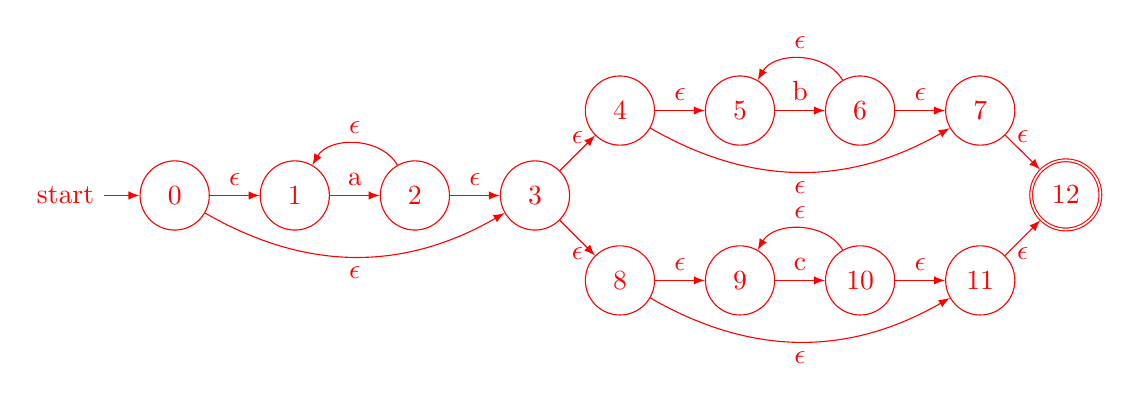
\begin{tikzpicture}[node distance=1.5pc,color=red]
\node[state,initial] (0) {0};
\node[state,right=of 0] (1) {1};
\node[state,right=of 1] (2) {2};
\node[state,right=of 2] (3) {3};
\node[state,above right=of 3] (4) {4};
\node[state,right=of 4] (5) {5};
\node[state,right=of 5] (6) {6};
\node[state,right=of 6] (7) {7};
\node[state,below right=of 3] (8) {8};
\node[state,right=of 8] (9) {9};
\node[state,right=of 9] (10) {10};
\node[state,right=of 10] (11) {11};
\node[state,accepting,above right=of 11] (12) {12};
\kleene 0 1 2 3
\single 1 2 a
\choice 3 4 8 7 {11} {12}
\kleene 4 5 6 7
\single 5 6 b
\kleene 8 9 {10} {11}
\single 9 {10} c
\end{tikzpicture}
}

\item (5 pts.) Convert the NFA you wrote in part (a) to a \textbf{DFA} using
  the \textbf{subset construction algorithm.}  \textbf{Fill in the table} below
  to show how you arrived at your DFA and \textbf{draw the DFA}.

  \hspace{-2.5pc}\myfbox{\textwidth}{2.75in}{
\renewcommand{\arraystretch}{1.5}\large
\ifkey\color{red}\fi
\begin{tabular}[b]{cp{14pc}ccc}
\toprule
\multicolumn{2}{@{}c@{}}{\textbf{Current State}} &
\multicolumn{3}{@{}c@{}}{\textbf{Next State}} \\
\cmidrule(r){1-2}
\cmidrule(l){3-5}
\textbf{DFA} &
\multicolumn{1}{@{\hspace{8pc}}c@{\hspace{8pc}}}{\textbf{NFA States}} &
\textbf{a} &
\textbf{b} &
\textbf{c} \\
\midrule
\ifkey
A & \{ 0, 1, 3, 4, 5, 7, 8, 9, 11, 12 \} & B & C & D \\
B & \{ 1, 2, 3, 4, 5, 7, 8, 9, 11, 12 \} & B & C & D  \\
C & \{ 5, 6, 7, 12 \} & & C & \\
D & \{ 9, 10, 11, 12 \} & & & D \\
\else
\\
\fi
\end{tabular}
\ifkey
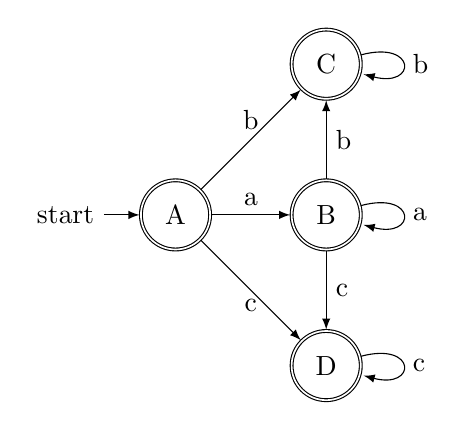
\begin{tikzpicture}
\node [state,initial,accepting] (A) {A};
\node [state,right=of A,accepting] (B) {B};
\node [state,above=of B,accepting] (C) {C};
\node [state,below=of B,accepting] (D) {D};
\path [->] (A) edge node [above] {a} (B)
           (A) edge node [above] {b} (C)
           (A) edge node [below] {c} (D)
           (B) edge node [right] {b} (C)
           (B) edge node [right] {c} (D)
           (B) edge [loop right] node [right] {a} ()
           (C) edge [loop right] node [right] {b} ()
           (D) edge [loop right] node [right] {c} ()
;
\end{tikzpicture}
\fi
}


\item (5 pts.) Show how your NFA from part (a) \textbf{accepts the
  string} $bb$ by indicating the \textbf{sequence of states} it goes
  through.

\def\trans#1{\buildrel{#1}\over\rightarrow}
\def\ep{\rightarrow}

\hspace{-2.5pc}\fullfield{0.5in}{
$0 \ep 3 \ep 4 \ep 5 \trans b 6 \ep 5 \trans b 6 \ep 7 \ep 12$
}

\item (5 pts.) Show how your DFA from part (b) \textbf{accepts the
  string} $bb$ by indicating the \textbf{sequence of states} it goes
  through.

\hspace{-2.5pc}\fullfield{0.5in}{
$A \trans b C \trans b C$
}

\end{enumerate}
\end{problem}

\newpage

\begin{problem}{8}{Normal vs. Applicative}

For the lambda term $(\lambda x . \lambda y . +\ y\ y)\ \big((\lambda z . z\ z)\ (\lambda w . w\ w)\big)$

\begin{enumerate}
\item (4 pts.) \textbf{Show the steps} in reducing this term to normal form, if
  possible, using \textbf{normal-order evaluation}. \\
  \textbf{Underline} the complete subexpression being $\beta$-reduced.

\hspace{-2.5pc}\fullfield{1.75in}{
$\underline{(\lambda x . \lambda y . +\ y\ y)\ \big((\lambda z . z\ z)\ (\lambda w . w\ w)\big)}$ 

$(\lambda y . +\ y\ y)$
}

\item (4 pts.) \textbf{Show the steps} in reducing this term to normal form, if
  possible, using \textbf{applicative order evaluation}.
  \textbf{Underline} each subexpression being $\beta$-reduced.

  \hspace{-2.5pc}\fullfield{1.75in}{
    $(\lambda x . \lambda y . +\ y\ y)\ \big(\underline{(\lambda z . z\ z)\ (\lambda w . w\ w)}\big)$


$(\lambda x . \lambda y . +\ y\ y)\ \big(\underline{(\lambda w . w\ w)\ (\lambda w . w\ w)}\big)$ 

Etc. Does not ever normalize.
}

\end{enumerate}

\end{problem}

\begin{problem}{15}{Church Numerals}
Recall the Church Numerals and the ``plus'' function, which adds \emph{m} to \emph{n}:

\medskip

\begin{lcalc}
0 & = & \lambda{f} . \lambda{x} . x \\
1 & = & \lambda{f} . \lambda{x} . f x \\
\end{lcalc}
\hfil
\begin{lcalc}
2 & = & \lambda{f} . \lambda{x} . f (f x) \\
3 & = & \lambda{f} . \lambda{x} . f \big(f (f x)\big) \\
\end{lcalc}
\hfil
\begin{lcalc}
\textrm{plus} & = & \lambda{m}.\lambda{n}.\lambda{f}.\lambda{x}. m f ( n f x)
\end{lcalc}

\medskip

\textbf{Prove} that in the Lambda Calculus, $\textrm{plus}\ 1\ 1 =
2$. \textbf{Justify} each step of your proof.

\noindent\fullfield{3in}{
\begin{lcalc}
\textrm{plus} 1 1 & = & (\lambda{m}.\lambda{n}.\lambda{f}.\lambda{x}. m f ( n f x)) 1 1 \\
& =_{\beta} & \lambda{f}.\lambda{x}. 1 f ( 1 f x )  \\
& = & \lambda{f}.\lambda{x}. 1 f ( (\lambda{f}. \lambda{x}. f x) f x ) \\
& =_{\beta} & \lambda{f}.\lambda{x}. 1 f ( f x ) \\
& = & \lambda{f}.\lambda{x}. (\lambda{f}. \lambda{x}. f x) f ( f x ) \\
& =_{\beta} & \lambda{f}.\lambda{x}. f ( f x ) \\
& = & 2 \\
\end{lcalc}
}


\end{problem}

\begin{problem}{25}{Parsers}
For the grammar \quad $\begin{array}{l}
E' \rightarrow E \\
E \rightarrow (\ E\ ) \\
E \rightarrow a
\end{array}$ \quad whose three terminals are (, ), and a.

\begin{enumerate}

\item (10 pts.) Complete its LR(0) automaton. Fill in the \textbf{items},
  indicate the \textbf{accepting states}, and label the
  \textbf{transitions}.  No additional transitions are necessary.

\newcommand{\itemtab}[1]{
  \ifkey{\color{red}
  \begin{tabular}{>{$}l<{$}@{\ $\rightarrow$\ }>{$}l<{$}} #1 
  \end{tabular}
}\fi}

\newcommand{\lab}[1]{\ifkey\textcolor{red}{#1}\fi}

\begin{tikzpicture}
\node [draw,minimum height=6pc,text width=10pc] (S0) {\itemtab{
E' & \cdot E \\
E & \cdot (\ E\ ) \\
E & \cdot a \\
}};

\node [draw,minimum height=6pc,text width=10pc,right=of S0] (S1) {\itemtab{
E' & E \cdot \\
}};

\node [draw,minimum height=6pc,text width=10pc,below right=of S0] (S2) {\itemtab{
E & ( \cdot E \ ) \\
E & \cdot (\ E\ ) \\
E & \cdot a \\
}};

\node [draw,minimum height=6pc,text width=10pc,left=of S2] (S3) {\itemtab{
E & a \cdot \\
}};

\node [draw,minimum height=6pc,text width=10pc,right=of S2,xshift=2pc] (S4) {\itemtab{
E & (\ E \cdot ) \\
}};

\node [draw,minimum height=6pc,text width=10pc,above=of S4] (S5) {\itemtab{
E & (\ E \ ) \cdot \\
}};

\node [below left] at (S0.north west) {S1};
\node [below left] at (S1.north west) {S6};
\node [below left] at (S2.north west) {S2};
\node [below left] at (S3.north west) {S3};
\node [below left] at (S4.north west) {S4};
\node [below left] at (S5.north west) {S5};

\path [<-] (S0.west) edge ++(left:0.5);

\path [->] (S0) edge node [above] {\lab E} (S1);
\path [->] (S0) edge node [above] {\lab (} (S2);
\path [->] (S0) edge node [right] {\lab{a}} (S3);
\path [->] (S2) edge [in=25,out=35,loop] node [right] {\lab (} ();
\path [->] (S2) edge node [above] {\lab{a}} (S3);
\path [->] (S2) edge node [above] {\lab{E}} (S4);
\path [->] (S4) edge node [right] {\lab )} (S5);

\end{tikzpicture}


\item (5 pts.) \textbf{Compute} the \textsc{first} and \textsc{follow} sets.  \textbf{Explain} your reasoning.

  \hspace{-2.5pc}\myfbox{\textwidth}{1.5in}{
\parskip=6pt

$\textsc{first}(E') = \Big\{ \ifkey{\color{red} (, a }\fi \hspace{10pc} \Big\}$

$\textsc{first}(E) = \Big\{ \ifkey{\color{red} (, a }\fi \hspace{10pc} \Big\}$


$\textsc{follow}(E') = \Big\{ \ifkey{\color{red} \$ }\fi \hspace{10pc} \Big\}$

$\textsc{follow}(E) = \Big\{ \ifkey{\color{red} ), \$ }\fi \hspace{10pc} \Big\}$

}

\item (10 pts.) \textbf{Fill in} the SLR parsing table:

\hspace{-2.5pc}\myfbox{\textwidth}{3in}{
\renewcommand{\arraystretch}{1.5}
\begin{tabular}{*{6}{p{3pc}}}
\toprule
\textbf{State} & \multicolumn{4}{c}{\textbf{Action}} & \textbf{Goto} \\
\cmidrule(lr){2-5}
\cmidrule(lr){6-6}
& \hfil ( & \hfil ) & \hfil a & \hfil\$ & \hfil E \\
\midrule
S1 & \ifkey \hfil s2 & \hfil  & \hfil  s3 & \hfil  & \hfil  6 \fi \\
\midrule
S2 & \ifkey \hfil s2 &  \hfil  & \hfil  s3 & \hfil  & \hfil  4 \fi \\
\midrule
S3 &  \ifkey &     \hfil  r2 & \hfil  & \hfil  r2 & \hfil  \fi \\
\midrule
S4 &  \ifkey &   \hfil  s5 & \hfil  & \hfil  & \hfil  \fi \\
\midrule
S5 &   \ifkey & \hfil  r1 & \hfil  & \hfil  r1 & \hfil  \fi \\
\midrule
S6 &   \ifkey & \hfil     & \hfil   & \hfil  acc & \hfil  \fi \\
\bottomrule
\end{tabular}
}

%\item Use your table to show the steps a shift/reduce parser would take parsing FIXME

\end{enumerate}
\end{problem}

\newpage

\begin{problem}{20}{Swift}
Swift is Apple's successor for Objective-C for iOS.  It blends
object-oriented and functional styles and includes such modern
features as type inference and closures.  The following program prints
what's shown on the right.

\medskip

\noindent
\begin{minipage}{0.7\textwidth}
  \small
\begin{verbatim}
func main() {
  var a = 5                 // Declare a mutable variable
  func b(_ i: Int) -> Int { // b is a function of a single argument
    print("i = \(i)")       // print the value of i
    a += i                  // add the argument to a
    return a
  }
  func go() {  
    func print3(x: Int, y: Int, z: Int) {
      print(x)
      print(x)
      print(z)
      print(y)
    }
    let a = 10              // Declare an immutable value
    print3(x: b(2), y: b(5), z: a);
  }

  go()                      // Body of main()
}

main()                      // Top level: call main()
\end{verbatim}
\end{minipage}
\rule[-10pc]{0.5pt}{20pc}
\quad
\begin{minipage}{0.2\textwidth}
\begin{verbatim}
i = 2
i = 5
7
7
10
12
\end{verbatim}
\end{minipage}

\renewcommand{\labelitemi}{$\square$}

\vspace{1.2\baselineskip}

\noindent
\textbf{Multiple choice:} Check one box per question

\begin{enumerate}
\begin{minipage}[t]{0.45\textwidth}
\item (5 pts.) Swift's \textbf{scoping policy} is

  \begin{itemize}
    \setlength\itemsep{0pt}
\item dynamic, because \emph{b} sees the first \emph{a} \key{+2}
\item dynamic, because \emph{b} returns the value of \emph{a} \key{+1}
\item static, because all the functions are defined \key{0}
\item static, because \emph{b} sees the first \emph{a} \key{+5}
\item impossible to tell from this example \key{0}
\end{itemize}
\end{minipage}
\begin{minipage}[t]{0.5\textwidth}
\item (5 pts.) This program indicates Swift's \textbf{evaluation order} is

  \begin{itemize}
    \setlength\itemsep{0pt}
\item applicative, because x, x, z, and y are printed in order \key{+3}
\item normal, because i = 2 and i = 5 are printed first \key{+2}
\item normal, because it is lazy \key{+1}
\item normal, because x, x, z, and y are printed in order \key{+1}
\item applicative, because i = 2 and i = 5 are printed first \key{+5}
\item impossible to tell from this example \key{0}
\end{itemize}
\end{minipage}

\vskip\baselineskip

\begin{minipage}[t]{0.45\textwidth}
\item (5 pts.) Based on this program, what can you say about \textbf{function activation records} in Swift?
  \begin{itemize}
            \setlength\itemsep{0pt}
\item All may be on the stack because only one version of \emph{a} is mutable. \key{0}
\item All may be on the stack because \emph{main} is active while
  \emph{b} is called. \key{+5}
\item Some must be on the heap because the outer \emph{a} is mutable.\key{+1}
\item Some must be on the heap because \emph{print3} is defined within
  \emph{go}. \key{+2}
\item All may be on the stack because \emph{print3} is defined within
  \emph{go}. \key{+3}
\item Some must be on the heap because \emph{b} references non-local
  variable \emph{a}. \key{+1}

\end{itemize}
\end{minipage}
\hfill
\begin{minipage}[t]{0.45\textwidth}
\item (5 pts.) Which function, if any, might use an \textbf{access (static)
  link} in its activation record?

  \begin{itemize}
    \setlength\itemsep{0pt}
\item \emph{b}, because it needs access to \emph{a} \key{+5}
\item \emph{go}, because it needs access to \emph{a} \key{+3}    
\item \emph{print3}, because it needs access to \emph{x}, \emph{y}, and \emph{z}\key{+1}
\item \emph{b}, because it needs access to \emph{print} \key{+2}
\item No function needs an access link \key{0}
\end{itemize}
\end{minipage}

\end{enumerate}

\end{problem}

\end{document}

% Local Variables:
% compile-command: "make final.pdf"
% End:


% Show succ 1 = 2
% RE ambiguity: what policy does the subset construction follow
"
% for solutions


% Compiler structure
% Scanning: RE, DFA, NFA, Subset construction
% Parsing: SLR table, shift/reduce parsing, First and Follow
% Types: arrays, structs and unions, static typing, polymorphism
% Runtime: activation records, recursion, variable-sized arrays, access links
%   Layout of structs, unions, arrays, malloc, reference counting, mark/sweep
%   Objects, inheritance, virtual functions
%   setjmp/longjmp, exceptions
% Code Generation: stack vs. register-based IRs, CFGs, optimization, linking
% Lambda Calculus: beta reduction, alpha conversion, normal form, Church-Rosser
%   Booleans, Church Numerals, Recursion and the Y combinator
% Prolog: Horn clauses, structures and functors, unification,
%   recursive searching, cuts

% ``Dismantle the following program into gotos, etc.''
% What does this Prolog program do?
% Strict functions and applicative order evaluation: what does this do?
% Unfamiliar language: scoping rules, applicative or normal order,

% Simple RE:
%
%  Draw NFA
%  Show parse of a string
%  Convert to DFA subset construction
%  Show parse of 
% 

% http://jsmachines.sourceforge.net/machines/slr.html
% Very simple grammar:
%
% E' -> E
% E -> ( E )
% E -> id
%
% six states
%
% Parse ( ( id ) )
%   steps: s2 s2 s3 r2 s5 r1 s5 r1
% 
%  Draw LR(0) automaton
%  First and follow sets
%  Fill in parse table
%  Parse simple input

% Draw parse trees for each way this expression could be parsed
%   Lambda calculus example

% Ocaml:
%   Is it applicative or normal?
%   Give a program, say it does this or that, and ask whether it's applicative
%   or normal
%
%   Can it use a stack for its activation records?
%    Simple example (yes)
%    Example that returns a lambda (no)


% Disambiguate a grammar by restructuring it
%
% E -> E + E | E ^ E | ( E ) | num
%
% make + left associative, ^ right associative, and + at a lower precedence
%
% E -> E + T | T
% T -> F ^ T | F
% F -> ( E ) | num

% Evaluate this lambda term using normal-order evaluation
%   " using applicative order evaluation

\usepackage[T1]{fontenc}
\usepackage{fourier}
\usepackage[scaled=0.88]{luximono}
\usepackage{booktabs}
\usepackage{array}
\usepackage{tikz}
\usetikzlibrary{positioning,calc,automata}
\usepackage{listings}
\lstset{basicstyle=\ttfamily}

{\obeyspaces\global\let =\ }
\newenvironment{lcalc}{\begingroup$\obeyspaces\begin{array}{r@{\;}c@{\;}l}}{\end{array}$\endgroup}

\newif\ifkey

%\def\showkey{}

\ifdefined\showkey
  \keytrue
\else
  \keyfalse
\fi

\newcommand{\key}[1]{\ifkey\rlap{\quad\textcolor{red}{#1}}\fi}

\newcommand{\fillinbox}[1][X]{%
  \framebox[3pc]{\rule[-1.2pc]{0pt}{3pc}\ifkey \textcolor{red}{\Large #1} \fi}\hspace{5pt}}

\makeatletter
\newcommand\listofproblems{
  \problemline{\textbf{Problem}}{\textbf{Value}}{\textbf{Score}}{\textbf{Description}}
  \@starttoc{lop}
  \problemline{Total}{\arabic{total}}{}{}
}
\makeatother

\def\labelenumi{\alph{enumi})}

\def\problemline#1#2#3#4{\noindent\par\hspace{10pc}\hbox{\hbox to 3.5pc{\hfil#1\hfil}\hbox to 3pc{\hfil#2\hfil}\hbox to 6pc{\hfil#3\hfil}\hbox{#4}}\par\noindent\hspace{10pc}\rule{23pc}{0.5pt}}

\def\problemspec#1#2#3#4{\problemline{#1}{#2}{#3}{#4}
\addtocounter{total}{#2}}

\newcounter{problem}
\newenvironment{problem}[2]{
  \refstepcounter{problem}
  \par\noindent
  \arabic{problem}. (#1 pts.)
  \addtocontents{lop}{\protect\problemspec{\theproblem}{#1}{}{#2}}
}

\newcounter{total}

% Make ``.'' a mathrel symbol: improves spacing in lambda expressions
\mathcode`\.="313A
% Make | a mathrel symbol
\mathcode`\|="326A

\tikzset{>=latex} % Nicer looking arrows

\usepackage[top=0.5in,bottom=1in,left=0.5in,right=0.5in]{geometry}

\def\kleene#1#2#3#4{
  \path [->] (#1) edge node [above] {$\epsilon$} (#2)
             (#3) edge node [above] {$\epsilon$} (#4)
             (#3) edge [bend right=60] node [above] {$\epsilon$} (#2)
             (#1) edge [bend right] node [below] {$\epsilon$} (#4)
  ;
}
\def\choice#1#2#3#4#5#6{
  \path [->] (#1) edge node [above] {$\epsilon$} (#2)
             (#1) edge node [below] {$\epsilon$} (#3)
             (#4) edge node [above] {$\epsilon$} (#6)
             (#5) edge node [below] {$\epsilon$} (#6)
  ;
}
\def\single#1#2#3{
  \path [->] (#1) edge node [above] {#3} (#2);
}

\newcommand{\myfbox}[3]{
  \fbox{\begin{minipage}[t][#2]{#1}\mbox{}#3\end{minipage}}
}

\newcommand{\field}[3]{
  \myfbox{#1}{#2}{\ifkey{\color{red}#3}\fi}
}

\def\fullfield{\field{\textwidth}}

\title{COMS W4115 Programming Languages and Translators Final}
\author{ Prof. Stephen A. Edwards \quad\quad December 10, 2018}
\date{}

\begin{document}
\maketitle

Name: \begin{tabular}{@{}c@{}}\field{30pc}{1.5pc}{Key}\end{tabular}
Uni: \begin{tabular}{@{}c@{}}\field{5pc}{1.5pc}{}\end{tabular}


{\parskip=0.5\baselineskip

  75 minutes
  
You may consult your own 8.5$''$ $\times$ 11$''$ double-sided sheet of
notes, but nothing else (e.g., no text, no other notes).

You may use a four-function calculator, but probably don't need one.

Put your answers in the boxes provided; writing outside the
boxes will not be graded.  Use scratch paper if necessary.

Explain your answers.

Check this box if you are \textbf{not enrolled} in the class (i.e.,
taking the comp exam)
\hspace{1pc}
\begin{tabular}{@{}c@{}}\field{0.7pc}{0.7pc}{}
\end{tabular}
}

\vspace{3pc}

%\listofproblems

% http://hackingoff.com/compilers/regular-expression-to-nfa-dfa

\begin{problem}{12}{Grammar Disambiguation}
Write an \textbf{unambiguous grammar} for the language defined by the
following ambiguous grammar by making the $+$ operator
\textbf{left-associative} and the $\wedge$ operator
\textbf{right-associative} at a \textbf{higher level of precedence}
than $+$. The terminals are $+$, $\wedge$, $($, $)$, and $n$.  $|$
indicates choice.

\[
E \rightarrow E + E | E \wedge E | (\ E\ ) | n
\]

\noindent\fullfield{2.5in}{
\[
\begin{array}{l}
E \rightarrow E + T \\
E \rightarrow T \\
T \rightarrow F \wedge T \\
T \rightarrow F \\
F \rightarrow ( E ) \\
F \rightarrow n
\end{array}
\]
}

\end{problem}

\newpage

\begin{problem}{20}{Regular Expressions}
\begin{enumerate}
\item (5 pts.) Using Thompson's construction (from class),
  \textbf{draw the NFA} for the regular expression $a^*|(b^*|c^*)$

\hspace{-2.5pc}\fullfield{2.75in}{
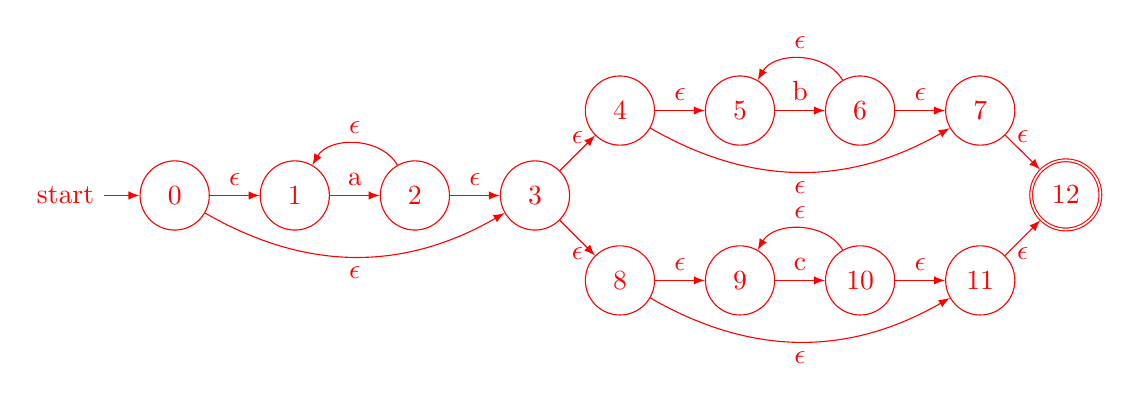
\begin{tikzpicture}[node distance=1.5pc,color=red]
\node[state,initial] (0) {0};
\node[state,right=of 0] (1) {1};
\node[state,right=of 1] (2) {2};
\node[state,right=of 2] (3) {3};
\node[state,above right=of 3] (4) {4};
\node[state,right=of 4] (5) {5};
\node[state,right=of 5] (6) {6};
\node[state,right=of 6] (7) {7};
\node[state,below right=of 3] (8) {8};
\node[state,right=of 8] (9) {9};
\node[state,right=of 9] (10) {10};
\node[state,right=of 10] (11) {11};
\node[state,accepting,above right=of 11] (12) {12};
\kleene 0 1 2 3
\single 1 2 a
\choice 3 4 8 7 {11} {12}
\kleene 4 5 6 7
\single 5 6 b
\kleene 8 9 {10} {11}
\single 9 {10} c
\end{tikzpicture}
}

\item (5 pts.) Convert the NFA you wrote in part (a) to a \textbf{DFA} using
  the \textbf{subset construction algorithm.}  \textbf{Fill in the table} below
  to show how you arrived at your DFA and \textbf{draw the DFA}.

  \hspace{-2.5pc}\myfbox{\textwidth}{2.75in}{
\renewcommand{\arraystretch}{1.5}\large
\ifkey\color{red}\fi
\begin{tabular}[b]{cp{14pc}ccc}
\toprule
\multicolumn{2}{@{}c@{}}{\textbf{Current State}} &
\multicolumn{3}{@{}c@{}}{\textbf{Next State}} \\
\cmidrule(r){1-2}
\cmidrule(l){3-5}
\textbf{DFA} &
\multicolumn{1}{@{\hspace{8pc}}c@{\hspace{8pc}}}{\textbf{NFA States}} &
\textbf{a} &
\textbf{b} &
\textbf{c} \\
\midrule
\ifkey
A & \{ 0, 1, 3, 4, 5, 7, 8, 9, 11, 12 \} & B & C & D \\
B & \{ 1, 2, 3, 4, 5, 7, 8, 9, 11, 12 \} & B & C & D  \\
C & \{ 5, 6, 7, 12 \} & & C & \\
D & \{ 9, 10, 11, 12 \} & & & D \\
\else
\\
\fi
\end{tabular}
\ifkey
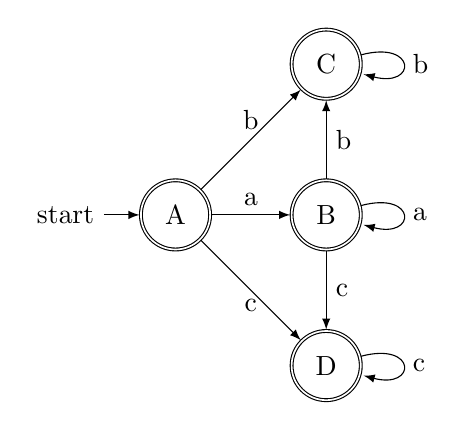
\begin{tikzpicture}
\node [state,initial,accepting] (A) {A};
\node [state,right=of A,accepting] (B) {B};
\node [state,above=of B,accepting] (C) {C};
\node [state,below=of B,accepting] (D) {D};
\path [->] (A) edge node [above] {a} (B)
           (A) edge node [above] {b} (C)
           (A) edge node [below] {c} (D)
           (B) edge node [right] {b} (C)
           (B) edge node [right] {c} (D)
           (B) edge [loop right] node [right] {a} ()
           (C) edge [loop right] node [right] {b} ()
           (D) edge [loop right] node [right] {c} ()
;
\end{tikzpicture}
\fi
}


\item (5 pts.) Show how your NFA from part (a) \textbf{accepts the
  string} $bb$ by indicating the \textbf{sequence of states} it goes
  through.

\def\trans#1{\buildrel{#1}\over\rightarrow}
\def\ep{\rightarrow}

\hspace{-2.5pc}\fullfield{0.5in}{
$0 \ep 3 \ep 4 \ep 5 \trans b 6 \ep 5 \trans b 6 \ep 7 \ep 12$
}

\item (5 pts.) Show how your DFA from part (b) \textbf{accepts the
  string} $bb$ by indicating the \textbf{sequence of states} it goes
  through.

\hspace{-2.5pc}\fullfield{0.5in}{
$A \trans b C \trans b C$
}

\end{enumerate}
\end{problem}

\newpage

\begin{problem}{8}{Normal vs. Applicative}

For the lambda term $(\lambda x . \lambda y . +\ y\ y)\ \big((\lambda z . z\ z)\ (\lambda w . w\ w)\big)$

\begin{enumerate}
\item (4 pts.) \textbf{Show the steps} in reducing this term to normal form, if
  possible, using \textbf{normal-order evaluation}. \\
  \textbf{Underline} the complete subexpression being $\beta$-reduced.

\hspace{-2.5pc}\fullfield{1.75in}{
$\underline{(\lambda x . \lambda y . +\ y\ y)\ \big((\lambda z . z\ z)\ (\lambda w . w\ w)\big)}$ 

$(\lambda y . +\ y\ y)$
}

\item (4 pts.) \textbf{Show the steps} in reducing this term to normal form, if
  possible, using \textbf{applicative order evaluation}.
  \textbf{Underline} each subexpression being $\beta$-reduced.

  \hspace{-2.5pc}\fullfield{1.75in}{
    $(\lambda x . \lambda y . +\ y\ y)\ \big(\underline{(\lambda z . z\ z)\ (\lambda w . w\ w)}\big)$


$(\lambda x . \lambda y . +\ y\ y)\ \big(\underline{(\lambda w . w\ w)\ (\lambda w . w\ w)}\big)$ 

Etc. Does not ever normalize.
}

\end{enumerate}

\end{problem}

\begin{problem}{15}{Church Numerals}
Recall the Church Numerals and the ``plus'' function, which adds \emph{m} to \emph{n}:

\medskip

\begin{lcalc}
0 & = & \lambda{f} . \lambda{x} . x \\
1 & = & \lambda{f} . \lambda{x} . f x \\
\end{lcalc}
\hfil
\begin{lcalc}
2 & = & \lambda{f} . \lambda{x} . f (f x) \\
3 & = & \lambda{f} . \lambda{x} . f \big(f (f x)\big) \\
\end{lcalc}
\hfil
\begin{lcalc}
\textrm{plus} & = & \lambda{m}.\lambda{n}.\lambda{f}.\lambda{x}. m f ( n f x)
\end{lcalc}

\medskip

\textbf{Prove} that in the Lambda Calculus, $\textrm{plus}\ 1\ 1 =
2$. \textbf{Justify} each step of your proof.

\noindent\fullfield{3in}{
\begin{lcalc}
\textrm{plus} 1 1 & = & (\lambda{m}.\lambda{n}.\lambda{f}.\lambda{x}. m f ( n f x)) 1 1 \\
& =_{\beta} & \lambda{f}.\lambda{x}. 1 f ( 1 f x )  \\
& = & \lambda{f}.\lambda{x}. 1 f ( (\lambda{f}. \lambda{x}. f x) f x ) \\
& =_{\beta} & \lambda{f}.\lambda{x}. 1 f ( f x ) \\
& = & \lambda{f}.\lambda{x}. (\lambda{f}. \lambda{x}. f x) f ( f x ) \\
& =_{\beta} & \lambda{f}.\lambda{x}. f ( f x ) \\
& = & 2 \\
\end{lcalc}
}


\end{problem}

\begin{problem}{25}{Parsers}
For the grammar \quad $\begin{array}{l}
E' \rightarrow E \\
E \rightarrow (\ E\ ) \\
E \rightarrow a
\end{array}$ \quad whose three terminals are (, ), and a.

\begin{enumerate}

\item (10 pts.) Complete its LR(0) automaton. Fill in the \textbf{items},
  indicate the \textbf{accepting states}, and label the
  \textbf{transitions}.  No additional transitions are necessary.

\newcommand{\itemtab}[1]{
  \ifkey{\color{red}
  \begin{tabular}{>{$}l<{$}@{\ $\rightarrow$\ }>{$}l<{$}} #1 
  \end{tabular}
}\fi}

\newcommand{\lab}[1]{\ifkey\textcolor{red}{#1}\fi}

\begin{tikzpicture}
\node [draw,minimum height=6pc,text width=10pc] (S0) {\itemtab{
E' & \cdot E \\
E & \cdot (\ E\ ) \\
E & \cdot a \\
}};

\node [draw,minimum height=6pc,text width=10pc,right=of S0] (S1) {\itemtab{
E' & E \cdot \\
}};

\node [draw,minimum height=6pc,text width=10pc,below right=of S0] (S2) {\itemtab{
E & ( \cdot E \ ) \\
E & \cdot (\ E\ ) \\
E & \cdot a \\
}};

\node [draw,minimum height=6pc,text width=10pc,left=of S2] (S3) {\itemtab{
E & a \cdot \\
}};

\node [draw,minimum height=6pc,text width=10pc,right=of S2,xshift=2pc] (S4) {\itemtab{
E & (\ E \cdot ) \\
}};

\node [draw,minimum height=6pc,text width=10pc,above=of S4] (S5) {\itemtab{
E & (\ E \ ) \cdot \\
}};

\node [below left] at (S0.north west) {S1};
\node [below left] at (S1.north west) {S6};
\node [below left] at (S2.north west) {S2};
\node [below left] at (S3.north west) {S3};
\node [below left] at (S4.north west) {S4};
\node [below left] at (S5.north west) {S5};

\path [<-] (S0.west) edge ++(left:0.5);

\path [->] (S0) edge node [above] {\lab E} (S1);
\path [->] (S0) edge node [above] {\lab (} (S2);
\path [->] (S0) edge node [right] {\lab{a}} (S3);
\path [->] (S2) edge [in=25,out=35,loop] node [right] {\lab (} ();
\path [->] (S2) edge node [above] {\lab{a}} (S3);
\path [->] (S2) edge node [above] {\lab{E}} (S4);
\path [->] (S4) edge node [right] {\lab )} (S5);

\end{tikzpicture}


\item (5 pts.) \textbf{Compute} the \textsc{first} and \textsc{follow} sets.  \textbf{Explain} your reasoning.

  \hspace{-2.5pc}\myfbox{\textwidth}{1.5in}{
\parskip=6pt

$\textsc{first}(E') = \Big\{ \ifkey{\color{red} (, a }\fi \hspace{10pc} \Big\}$

$\textsc{first}(E) = \Big\{ \ifkey{\color{red} (, a }\fi \hspace{10pc} \Big\}$


$\textsc{follow}(E') = \Big\{ \ifkey{\color{red} \$ }\fi \hspace{10pc} \Big\}$

$\textsc{follow}(E) = \Big\{ \ifkey{\color{red} ), \$ }\fi \hspace{10pc} \Big\}$

}

\item (10 pts.) \textbf{Fill in} the SLR parsing table:

\hspace{-2.5pc}\myfbox{\textwidth}{3in}{
\renewcommand{\arraystretch}{1.5}
\begin{tabular}{*{6}{p{3pc}}}
\toprule
\textbf{State} & \multicolumn{4}{c}{\textbf{Action}} & \textbf{Goto} \\
\cmidrule(lr){2-5}
\cmidrule(lr){6-6}
& \hfil ( & \hfil ) & \hfil a & \hfil\$ & \hfil E \\
\midrule
S1 & \ifkey \hfil s2 & \hfil  & \hfil  s3 & \hfil  & \hfil  6 \fi \\
\midrule
S2 & \ifkey \hfil s2 &  \hfil  & \hfil  s3 & \hfil  & \hfil  4 \fi \\
\midrule
S3 &  \ifkey &     \hfil  r2 & \hfil  & \hfil  r2 & \hfil  \fi \\
\midrule
S4 &  \ifkey &   \hfil  s5 & \hfil  & \hfil  & \hfil  \fi \\
\midrule
S5 &   \ifkey & \hfil  r1 & \hfil  & \hfil  r1 & \hfil  \fi \\
\midrule
S6 &   \ifkey & \hfil     & \hfil   & \hfil  acc & \hfil  \fi \\
\bottomrule
\end{tabular}
}

%\item Use your table to show the steps a shift/reduce parser would take parsing FIXME

\end{enumerate}
\end{problem}

\newpage

\begin{problem}{20}{Swift}
Swift is Apple's successor for Objective-C for iOS.  It blends
object-oriented and functional styles and includes such modern
features as type inference and closures.  The following program prints
what's shown on the right.

\medskip

\noindent
\begin{minipage}{0.7\textwidth}
  \small
\begin{verbatim}
func main() {
  var a = 5                 // Declare a mutable variable
  func b(_ i: Int) -> Int { // b is a function of a single argument
    print("i = \(i)")       // print the value of i
    a += i                  // add the argument to a
    return a
  }
  func go() {  
    func print3(x: Int, y: Int, z: Int) {
      print(x)
      print(x)
      print(z)
      print(y)
    }
    let a = 10              // Declare an immutable value
    print3(x: b(2), y: b(5), z: a);
  }

  go()                      // Body of main()
}

main()                      // Top level: call main()
\end{verbatim}
\end{minipage}
\rule[-10pc]{0.5pt}{20pc}
\quad
\begin{minipage}{0.2\textwidth}
\begin{verbatim}
i = 2
i = 5
7
7
10
12
\end{verbatim}
\end{minipage}

\renewcommand{\labelitemi}{$\square$}

\vspace{1.2\baselineskip}

\noindent
\textbf{Multiple choice:} Check one box per question

\begin{enumerate}
\begin{minipage}[t]{0.45\textwidth}
\item (5 pts.) Swift's \textbf{scoping policy} is

  \begin{itemize}
    \setlength\itemsep{0pt}
\item dynamic, because \emph{b} sees the first \emph{a} \key{+2}
\item dynamic, because \emph{b} returns the value of \emph{a} \key{+1}
\item static, because all the functions are defined \key{0}
\item static, because \emph{b} sees the first \emph{a} \key{+5}
\item impossible to tell from this example \key{0}
\end{itemize}
\end{minipage}
\begin{minipage}[t]{0.5\textwidth}
\item (5 pts.) This program indicates Swift's \textbf{evaluation order} is

  \begin{itemize}
    \setlength\itemsep{0pt}
\item applicative, because x, x, z, and y are printed in order \key{+3}
\item normal, because i = 2 and i = 5 are printed first \key{+2}
\item normal, because it is lazy \key{+1}
\item normal, because x, x, z, and y are printed in order \key{+1}
\item applicative, because i = 2 and i = 5 are printed first \key{+5}
\item impossible to tell from this example \key{0}
\end{itemize}
\end{minipage}

\vskip\baselineskip

\begin{minipage}[t]{0.45\textwidth}
\item (5 pts.) Based on this program, what can you say about \textbf{function activation records} in Swift?
  \begin{itemize}
            \setlength\itemsep{0pt}
\item All may be on the stack because only one version of \emph{a} is mutable. \key{0}
\item All may be on the stack because \emph{main} is active while
  \emph{b} is called. \key{+5}
\item Some must be on the heap because the outer \emph{a} is mutable.\key{+1}
\item Some must be on the heap because \emph{print3} is defined within
  \emph{go}. \key{+2}
\item All may be on the stack because \emph{print3} is defined within
  \emph{go}. \key{+3}
\item Some must be on the heap because \emph{b} references non-local
  variable \emph{a}. \key{+1}

\end{itemize}
\end{minipage}
\hfill
\begin{minipage}[t]{0.45\textwidth}
\item (5 pts.) Which function, if any, might use an \textbf{access (static)
  link} in its activation record?

  \begin{itemize}
    \setlength\itemsep{0pt}
\item \emph{b}, because it needs access to \emph{a} \key{+5}
\item \emph{go}, because it needs access to \emph{a} \key{+3}    
\item \emph{print3}, because it needs access to \emph{x}, \emph{y}, and \emph{z}\key{+1}
\item \emph{b}, because it needs access to \emph{print} \key{+2}
\item No function needs an access link \key{0}
\end{itemize}
\end{minipage}

\end{enumerate}

\end{problem}

\end{document}

% Local Variables:
% compile-command: "make final.pdf"
% End:


% Show succ 1 = 2
% RE ambiguity: what policy does the subset construction follow
"
% for solutions


% Compiler structure
% Scanning: RE, DFA, NFA, Subset construction
% Parsing: SLR table, shift/reduce parsing, First and Follow
% Types: arrays, structs and unions, static typing, polymorphism
% Runtime: activation records, recursion, variable-sized arrays, access links
%   Layout of structs, unions, arrays, malloc, reference counting, mark/sweep
%   Objects, inheritance, virtual functions
%   setjmp/longjmp, exceptions
% Code Generation: stack vs. register-based IRs, CFGs, optimization, linking
% Lambda Calculus: beta reduction, alpha conversion, normal form, Church-Rosser
%   Booleans, Church Numerals, Recursion and the Y combinator
% Prolog: Horn clauses, structures and functors, unification,
%   recursive searching, cuts

% ``Dismantle the following program into gotos, etc.''
% What does this Prolog program do?
% Strict functions and applicative order evaluation: what does this do?
% Unfamiliar language: scoping rules, applicative or normal order,

% Simple RE:
%
%  Draw NFA
%  Show parse of a string
%  Convert to DFA subset construction
%  Show parse of 
% 

% http://jsmachines.sourceforge.net/machines/slr.html
% Very simple grammar:
%
% E' -> E
% E -> ( E )
% E -> id
%
% six states
%
% Parse ( ( id ) )
%   steps: s2 s2 s3 r2 s5 r1 s5 r1
% 
%  Draw LR(0) automaton
%  First and follow sets
%  Fill in parse table
%  Parse simple input

% Draw parse trees for each way this expression could be parsed
%   Lambda calculus example

% Ocaml:
%   Is it applicative or normal?
%   Give a program, say it does this or that, and ask whether it's applicative
%   or normal
%
%   Can it use a stack for its activation records?
%    Simple example (yes)
%    Example that returns a lambda (no)


% Disambiguate a grammar by restructuring it
%
% E -> E + E | E ^ E | ( E ) | num
%
% make + left associative, ^ right associative, and + at a lower precedence
%
% E -> E + T | T
% T -> F ^ T | F
% F -> ( E ) | num

% Evaluate this lambda term using normal-order evaluation
%   " using applicative order evaluation

\usepackage[T1]{fontenc}
\usepackage{fourier}
\usepackage[scaled=0.88]{luximono}
\usepackage{booktabs}
\usepackage{array}
\usepackage{tikz}
\usetikzlibrary{positioning,calc,automata}
\usepackage{listings}
\lstset{basicstyle=\ttfamily}

{\obeyspaces\global\let =\ }
\newenvironment{lcalc}{\begingroup$\obeyspaces\begin{array}{r@{\;}c@{\;}l}}{\end{array}$\endgroup}

\newif\ifkey

%\def\showkey{}

\ifdefined\showkey
  \keytrue
\else
  \keyfalse
\fi

\newcommand{\key}[1]{\ifkey\rlap{\quad\textcolor{red}{#1}}\fi}

\newcommand{\fillinbox}[1][X]{%
  \framebox[3pc]{\rule[-1.2pc]{0pt}{3pc}\ifkey \textcolor{red}{\Large #1} \fi}\hspace{5pt}}

\makeatletter
\newcommand\listofproblems{
  \problemline{\textbf{Problem}}{\textbf{Value}}{\textbf{Score}}{\textbf{Description}}
  \@starttoc{lop}
  \problemline{Total}{\arabic{total}}{}{}
}
\makeatother

\def\labelenumi{\alph{enumi})}

\def\problemline#1#2#3#4{\noindent\par\hspace{10pc}\hbox{\hbox to 3.5pc{\hfil#1\hfil}\hbox to 3pc{\hfil#2\hfil}\hbox to 6pc{\hfil#3\hfil}\hbox{#4}}\par\noindent\hspace{10pc}\rule{23pc}{0.5pt}}

\def\problemspec#1#2#3#4{\problemline{#1}{#2}{#3}{#4}
\addtocounter{total}{#2}}

\newcounter{problem}
\newenvironment{problem}[2]{
  \refstepcounter{problem}
  \par\noindent
  \arabic{problem}. (#1 pts.)
  \addtocontents{lop}{\protect\problemspec{\theproblem}{#1}{}{#2}}
}

\newcounter{total}

% Make ``.'' a mathrel symbol: improves spacing in lambda expressions
\mathcode`\.="313A
% Make | a mathrel symbol
\mathcode`\|="326A

\tikzset{>=latex} % Nicer looking arrows

\usepackage[top=0.5in,bottom=1in,left=0.5in,right=0.5in]{geometry}

\def\kleene#1#2#3#4{
  \path [->] (#1) edge node [above] {$\epsilon$} (#2)
             (#3) edge node [above] {$\epsilon$} (#4)
             (#3) edge [bend right=60] node [above] {$\epsilon$} (#2)
             (#1) edge [bend right] node [below] {$\epsilon$} (#4)
  ;
}
\def\choice#1#2#3#4#5#6{
  \path [->] (#1) edge node [above] {$\epsilon$} (#2)
             (#1) edge node [below] {$\epsilon$} (#3)
             (#4) edge node [above] {$\epsilon$} (#6)
             (#5) edge node [below] {$\epsilon$} (#6)
  ;
}
\def\single#1#2#3{
  \path [->] (#1) edge node [above] {#3} (#2);
}

\newcommand{\myfbox}[3]{
  \fbox{\begin{minipage}[t][#2]{#1}\mbox{}#3\end{minipage}}
}

\newcommand{\field}[3]{
  \myfbox{#1}{#2}{\ifkey{\color{red}#3}\fi}
}

\def\fullfield{\field{\textwidth}}

\title{COMS W4115 Programming Languages and Translators Final}
\author{ Prof. Stephen A. Edwards \quad\quad December 10, 2018}
\date{}

\begin{document}
\maketitle

Name: \begin{tabular}{@{}c@{}}\field{30pc}{1.5pc}{Key}\end{tabular}
Uni: \begin{tabular}{@{}c@{}}\field{5pc}{1.5pc}{}\end{tabular}


{\parskip=0.5\baselineskip

  75 minutes
  
You may consult your own 8.5$''$ $\times$ 11$''$ double-sided sheet of
notes, but nothing else (e.g., no text, no other notes).

You may use a four-function calculator, but probably don't need one.

Put your answers in the boxes provided; writing outside the
boxes will not be graded.  Use scratch paper if necessary.

Explain your answers.

Check this box if you are \textbf{not enrolled} in the class (i.e.,
taking the comp exam)
\hspace{1pc}
\begin{tabular}{@{}c@{}}\field{0.7pc}{0.7pc}{}
\end{tabular}
}

\vspace{3pc}

%\listofproblems

% http://hackingoff.com/compilers/regular-expression-to-nfa-dfa

\begin{problem}{12}{Grammar Disambiguation}
Write an \textbf{unambiguous grammar} for the language defined by the
following ambiguous grammar by making the $+$ operator
\textbf{left-associative} and the $\wedge$ operator
\textbf{right-associative} at a \textbf{higher level of precedence}
than $+$. The terminals are $+$, $\wedge$, $($, $)$, and $n$.  $|$
indicates choice.

\[
E \rightarrow E + E | E \wedge E | (\ E\ ) | n
\]

\noindent\fullfield{2.5in}{
\[
\begin{array}{l}
E \rightarrow E + T \\
E \rightarrow T \\
T \rightarrow F \wedge T \\
T \rightarrow F \\
F \rightarrow ( E ) \\
F \rightarrow n
\end{array}
\]
}

\end{problem}

\newpage

\begin{problem}{20}{Regular Expressions}
\begin{enumerate}
\item (5 pts.) Using Thompson's construction (from class),
  \textbf{draw the NFA} for the regular expression $a^*|(b^*|c^*)$

\hspace{-2.5pc}\fullfield{2.75in}{
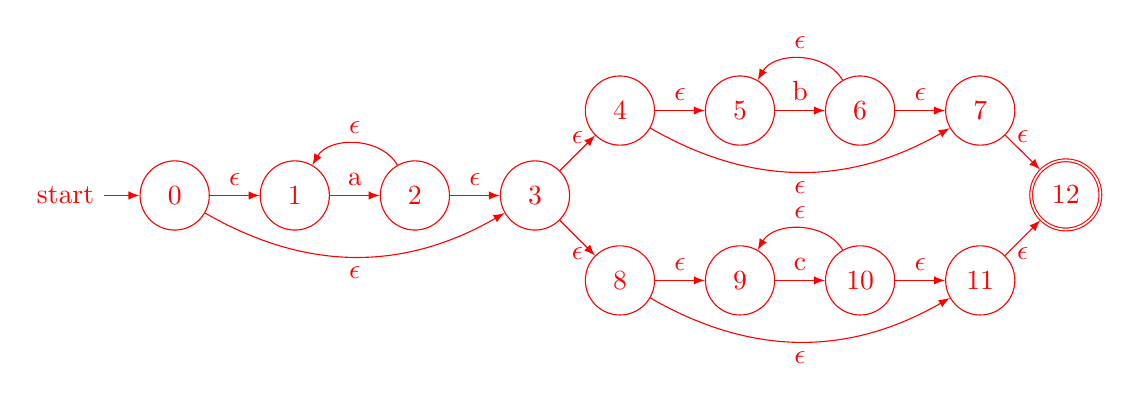
\begin{tikzpicture}[node distance=1.5pc,color=red]
\node[state,initial] (0) {0};
\node[state,right=of 0] (1) {1};
\node[state,right=of 1] (2) {2};
\node[state,right=of 2] (3) {3};
\node[state,above right=of 3] (4) {4};
\node[state,right=of 4] (5) {5};
\node[state,right=of 5] (6) {6};
\node[state,right=of 6] (7) {7};
\node[state,below right=of 3] (8) {8};
\node[state,right=of 8] (9) {9};
\node[state,right=of 9] (10) {10};
\node[state,right=of 10] (11) {11};
\node[state,accepting,above right=of 11] (12) {12};
\kleene 0 1 2 3
\single 1 2 a
\choice 3 4 8 7 {11} {12}
\kleene 4 5 6 7
\single 5 6 b
\kleene 8 9 {10} {11}
\single 9 {10} c
\end{tikzpicture}
}

\item (5 pts.) Convert the NFA you wrote in part (a) to a \textbf{DFA} using
  the \textbf{subset construction algorithm.}  \textbf{Fill in the table} below
  to show how you arrived at your DFA and \textbf{draw the DFA}.

  \hspace{-2.5pc}\myfbox{\textwidth}{2.75in}{
\renewcommand{\arraystretch}{1.5}\large
\ifkey\color{red}\fi
\begin{tabular}[b]{cp{14pc}ccc}
\toprule
\multicolumn{2}{@{}c@{}}{\textbf{Current State}} &
\multicolumn{3}{@{}c@{}}{\textbf{Next State}} \\
\cmidrule(r){1-2}
\cmidrule(l){3-5}
\textbf{DFA} &
\multicolumn{1}{@{\hspace{8pc}}c@{\hspace{8pc}}}{\textbf{NFA States}} &
\textbf{a} &
\textbf{b} &
\textbf{c} \\
\midrule
\ifkey
A & \{ 0, 1, 3, 4, 5, 7, 8, 9, 11, 12 \} & B & C & D \\
B & \{ 1, 2, 3, 4, 5, 7, 8, 9, 11, 12 \} & B & C & D  \\
C & \{ 5, 6, 7, 12 \} & & C & \\
D & \{ 9, 10, 11, 12 \} & & & D \\
\else
\\
\fi
\end{tabular}
\ifkey
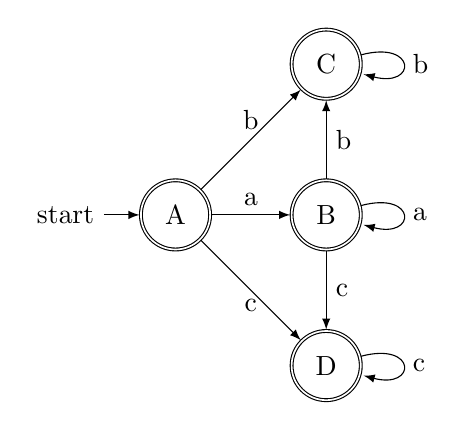
\begin{tikzpicture}
\node [state,initial,accepting] (A) {A};
\node [state,right=of A,accepting] (B) {B};
\node [state,above=of B,accepting] (C) {C};
\node [state,below=of B,accepting] (D) {D};
\path [->] (A) edge node [above] {a} (B)
           (A) edge node [above] {b} (C)
           (A) edge node [below] {c} (D)
           (B) edge node [right] {b} (C)
           (B) edge node [right] {c} (D)
           (B) edge [loop right] node [right] {a} ()
           (C) edge [loop right] node [right] {b} ()
           (D) edge [loop right] node [right] {c} ()
;
\end{tikzpicture}
\fi
}


\item (5 pts.) Show how your NFA from part (a) \textbf{accepts the
  string} $bb$ by indicating the \textbf{sequence of states} it goes
  through.

\def\trans#1{\buildrel{#1}\over\rightarrow}
\def\ep{\rightarrow}

\hspace{-2.5pc}\fullfield{0.5in}{
$0 \ep 3 \ep 4 \ep 5 \trans b 6 \ep 5 \trans b 6 \ep 7 \ep 12$
}

\item (5 pts.) Show how your DFA from part (b) \textbf{accepts the
  string} $bb$ by indicating the \textbf{sequence of states} it goes
  through.

\hspace{-2.5pc}\fullfield{0.5in}{
$A \trans b C \trans b C$
}

\end{enumerate}
\end{problem}

\newpage

\begin{problem}{8}{Normal vs. Applicative}

For the lambda term $(\lambda x . \lambda y . +\ y\ y)\ \big((\lambda z . z\ z)\ (\lambda w . w\ w)\big)$

\begin{enumerate}
\item (4 pts.) \textbf{Show the steps} in reducing this term to normal form, if
  possible, using \textbf{normal-order evaluation}. \\
  \textbf{Underline} the complete subexpression being $\beta$-reduced.

\hspace{-2.5pc}\fullfield{1.75in}{
$\underline{(\lambda x . \lambda y . +\ y\ y)\ \big((\lambda z . z\ z)\ (\lambda w . w\ w)\big)}$ 

$(\lambda y . +\ y\ y)$
}

\item (4 pts.) \textbf{Show the steps} in reducing this term to normal form, if
  possible, using \textbf{applicative order evaluation}.
  \textbf{Underline} each subexpression being $\beta$-reduced.

  \hspace{-2.5pc}\fullfield{1.75in}{
    $(\lambda x . \lambda y . +\ y\ y)\ \big(\underline{(\lambda z . z\ z)\ (\lambda w . w\ w)}\big)$


$(\lambda x . \lambda y . +\ y\ y)\ \big(\underline{(\lambda w . w\ w)\ (\lambda w . w\ w)}\big)$ 

Etc. Does not ever normalize.
}

\end{enumerate}

\end{problem}

\begin{problem}{15}{Church Numerals}
Recall the Church Numerals and the ``plus'' function, which adds \emph{m} to \emph{n}:

\medskip

\begin{lcalc}
0 & = & \lambda{f} . \lambda{x} . x \\
1 & = & \lambda{f} . \lambda{x} . f x \\
\end{lcalc}
\hfil
\begin{lcalc}
2 & = & \lambda{f} . \lambda{x} . f (f x) \\
3 & = & \lambda{f} . \lambda{x} . f \big(f (f x)\big) \\
\end{lcalc}
\hfil
\begin{lcalc}
\textrm{plus} & = & \lambda{m}.\lambda{n}.\lambda{f}.\lambda{x}. m f ( n f x)
\end{lcalc}

\medskip

\textbf{Prove} that in the Lambda Calculus, $\textrm{plus}\ 1\ 1 =
2$. \textbf{Justify} each step of your proof.

\noindent\fullfield{3in}{
\begin{lcalc}
\textrm{plus} 1 1 & = & (\lambda{m}.\lambda{n}.\lambda{f}.\lambda{x}. m f ( n f x)) 1 1 \\
& =_{\beta} & \lambda{f}.\lambda{x}. 1 f ( 1 f x )  \\
& = & \lambda{f}.\lambda{x}. 1 f ( (\lambda{f}. \lambda{x}. f x) f x ) \\
& =_{\beta} & \lambda{f}.\lambda{x}. 1 f ( f x ) \\
& = & \lambda{f}.\lambda{x}. (\lambda{f}. \lambda{x}. f x) f ( f x ) \\
& =_{\beta} & \lambda{f}.\lambda{x}. f ( f x ) \\
& = & 2 \\
\end{lcalc}
}


\end{problem}

\begin{problem}{25}{Parsers}
For the grammar \quad $\begin{array}{l}
E' \rightarrow E \\
E \rightarrow (\ E\ ) \\
E \rightarrow a
\end{array}$ \quad whose three terminals are (, ), and a.

\begin{enumerate}

\item (10 pts.) Complete its LR(0) automaton. Fill in the \textbf{items},
  indicate the \textbf{accepting states}, and label the
  \textbf{transitions}.  No additional transitions are necessary.

\newcommand{\itemtab}[1]{
  \ifkey{\color{red}
  \begin{tabular}{>{$}l<{$}@{\ $\rightarrow$\ }>{$}l<{$}} #1 
  \end{tabular}
}\fi}

\newcommand{\lab}[1]{\ifkey\textcolor{red}{#1}\fi}

\begin{tikzpicture}
\node [draw,minimum height=6pc,text width=10pc] (S0) {\itemtab{
E' & \cdot E \\
E & \cdot (\ E\ ) \\
E & \cdot a \\
}};

\node [draw,minimum height=6pc,text width=10pc,right=of S0] (S1) {\itemtab{
E' & E \cdot \\
}};

\node [draw,minimum height=6pc,text width=10pc,below right=of S0] (S2) {\itemtab{
E & ( \cdot E \ ) \\
E & \cdot (\ E\ ) \\
E & \cdot a \\
}};

\node [draw,minimum height=6pc,text width=10pc,left=of S2] (S3) {\itemtab{
E & a \cdot \\
}};

\node [draw,minimum height=6pc,text width=10pc,right=of S2,xshift=2pc] (S4) {\itemtab{
E & (\ E \cdot ) \\
}};

\node [draw,minimum height=6pc,text width=10pc,above=of S4] (S5) {\itemtab{
E & (\ E \ ) \cdot \\
}};

\node [below left] at (S0.north west) {S1};
\node [below left] at (S1.north west) {S6};
\node [below left] at (S2.north west) {S2};
\node [below left] at (S3.north west) {S3};
\node [below left] at (S4.north west) {S4};
\node [below left] at (S5.north west) {S5};

\path [<-] (S0.west) edge ++(left:0.5);

\path [->] (S0) edge node [above] {\lab E} (S1);
\path [->] (S0) edge node [above] {\lab (} (S2);
\path [->] (S0) edge node [right] {\lab{a}} (S3);
\path [->] (S2) edge [in=25,out=35,loop] node [right] {\lab (} ();
\path [->] (S2) edge node [above] {\lab{a}} (S3);
\path [->] (S2) edge node [above] {\lab{E}} (S4);
\path [->] (S4) edge node [right] {\lab )} (S5);

\end{tikzpicture}


\item (5 pts.) \textbf{Compute} the \textsc{first} and \textsc{follow} sets.  \textbf{Explain} your reasoning.

  \hspace{-2.5pc}\myfbox{\textwidth}{1.5in}{
\parskip=6pt

$\textsc{first}(E') = \Big\{ \ifkey{\color{red} (, a }\fi \hspace{10pc} \Big\}$

$\textsc{first}(E) = \Big\{ \ifkey{\color{red} (, a }\fi \hspace{10pc} \Big\}$


$\textsc{follow}(E') = \Big\{ \ifkey{\color{red} \$ }\fi \hspace{10pc} \Big\}$

$\textsc{follow}(E) = \Big\{ \ifkey{\color{red} ), \$ }\fi \hspace{10pc} \Big\}$

}

\item (10 pts.) \textbf{Fill in} the SLR parsing table:

\hspace{-2.5pc}\myfbox{\textwidth}{3in}{
\renewcommand{\arraystretch}{1.5}
\begin{tabular}{*{6}{p{3pc}}}
\toprule
\textbf{State} & \multicolumn{4}{c}{\textbf{Action}} & \textbf{Goto} \\
\cmidrule(lr){2-5}
\cmidrule(lr){6-6}
& \hfil ( & \hfil ) & \hfil a & \hfil\$ & \hfil E \\
\midrule
S1 & \ifkey \hfil s2 & \hfil  & \hfil  s3 & \hfil  & \hfil  6 \fi \\
\midrule
S2 & \ifkey \hfil s2 &  \hfil  & \hfil  s3 & \hfil  & \hfil  4 \fi \\
\midrule
S3 &  \ifkey &     \hfil  r2 & \hfil  & \hfil  r2 & \hfil  \fi \\
\midrule
S4 &  \ifkey &   \hfil  s5 & \hfil  & \hfil  & \hfil  \fi \\
\midrule
S5 &   \ifkey & \hfil  r1 & \hfil  & \hfil  r1 & \hfil  \fi \\
\midrule
S6 &   \ifkey & \hfil     & \hfil   & \hfil  acc & \hfil  \fi \\
\bottomrule
\end{tabular}
}

%\item Use your table to show the steps a shift/reduce parser would take parsing FIXME

\end{enumerate}
\end{problem}

\newpage

\begin{problem}{20}{Swift}
Swift is Apple's successor for Objective-C for iOS.  It blends
object-oriented and functional styles and includes such modern
features as type inference and closures.  The following program prints
what's shown on the right.

\medskip

\noindent
\begin{minipage}{0.7\textwidth}
  \small
\begin{verbatim}
func main() {
  var a = 5                 // Declare a mutable variable
  func b(_ i: Int) -> Int { // b is a function of a single argument
    print("i = \(i)")       // print the value of i
    a += i                  // add the argument to a
    return a
  }
  func go() {  
    func print3(x: Int, y: Int, z: Int) {
      print(x)
      print(x)
      print(z)
      print(y)
    }
    let a = 10              // Declare an immutable value
    print3(x: b(2), y: b(5), z: a);
  }

  go()                      // Body of main()
}

main()                      // Top level: call main()
\end{verbatim}
\end{minipage}
\rule[-10pc]{0.5pt}{20pc}
\quad
\begin{minipage}{0.2\textwidth}
\begin{verbatim}
i = 2
i = 5
7
7
10
12
\end{verbatim}
\end{minipage}

\renewcommand{\labelitemi}{$\square$}

\vspace{1.2\baselineskip}

\noindent
\textbf{Multiple choice:} Check one box per question

\begin{enumerate}
\begin{minipage}[t]{0.45\textwidth}
\item (5 pts.) Swift's \textbf{scoping policy} is

  \begin{itemize}
    \setlength\itemsep{0pt}
\item dynamic, because \emph{b} sees the first \emph{a} \key{+2}
\item dynamic, because \emph{b} returns the value of \emph{a} \key{+1}
\item static, because all the functions are defined \key{0}
\item static, because \emph{b} sees the first \emph{a} \key{+5}
\item impossible to tell from this example \key{0}
\end{itemize}
\end{minipage}
\begin{minipage}[t]{0.5\textwidth}
\item (5 pts.) This program indicates Swift's \textbf{evaluation order} is

  \begin{itemize}
    \setlength\itemsep{0pt}
\item applicative, because x, x, z, and y are printed in order \key{+3}
\item normal, because i = 2 and i = 5 are printed first \key{+2}
\item normal, because it is lazy \key{+1}
\item normal, because x, x, z, and y are printed in order \key{+1}
\item applicative, because i = 2 and i = 5 are printed first \key{+5}
\item impossible to tell from this example \key{0}
\end{itemize}
\end{minipage}

\vskip\baselineskip

\begin{minipage}[t]{0.45\textwidth}
\item (5 pts.) Based on this program, what can you say about \textbf{function activation records} in Swift?
  \begin{itemize}
            \setlength\itemsep{0pt}
\item All may be on the stack because only one version of \emph{a} is mutable. \key{0}
\item All may be on the stack because \emph{main} is active while
  \emph{b} is called. \key{+5}
\item Some must be on the heap because the outer \emph{a} is mutable.\key{+1}
\item Some must be on the heap because \emph{print3} is defined within
  \emph{go}. \key{+2}
\item All may be on the stack because \emph{print3} is defined within
  \emph{go}. \key{+3}
\item Some must be on the heap because \emph{b} references non-local
  variable \emph{a}. \key{+1}

\end{itemize}
\end{minipage}
\hfill
\begin{minipage}[t]{0.45\textwidth}
\item (5 pts.) Which function, if any, might use an \textbf{access (static)
  link} in its activation record?

  \begin{itemize}
    \setlength\itemsep{0pt}
\item \emph{b}, because it needs access to \emph{a} \key{+5}
\item \emph{go}, because it needs access to \emph{a} \key{+3}    
\item \emph{print3}, because it needs access to \emph{x}, \emph{y}, and \emph{z}\key{+1}
\item \emph{b}, because it needs access to \emph{print} \key{+2}
\item No function needs an access link \key{0}
\end{itemize}
\end{minipage}

\end{enumerate}

\end{problem}

\end{document}

% Local Variables:
% compile-command: "make final.pdf"
% End:


% Show succ 1 = 2
% RE ambiguity: what policy does the subset construction follow
